\documentclass[11pt]{article}
\usepackage{tocloft}
\usepackage{graphicx}
\usepackage{calc}
\usepackage{amssymb}
\usepackage{color}
\usepackage[sc]{mathpazo}
\usepackage{url}

%\linespread{1.05}
\oddsidemargin=0pt
\evensidemargin=0pt
\textwidth=6.5in
\topmargin=0pt
\headheight=0pt
\headsep=0pt
\textheight=9in
% EXPERIMENTAL
%\parindent=0pt
%\parskip=3pt
\setlength{\parindent}{0cm}
\newcommand\secfont{\fontfamily{cmss}\selectfont}%\textwidth 5.5truein
\newcommand\pifheading[1]{{\secfont\textbf{#1}:}}
%\oddsidemargin -0.40truein
%\textheight 8.0truein
%\topmargin -0.25truein
\def\lo{
\mathrel{\raise.3ex\hbox{$<$}\mkern-14mu\lower0.6ex\hbox{$\sim$}}
}
\def\hi{
\mathrel{\raise.3ex\hbox{$>$}\mkern-14mu\lower0.6ex\hbox{$\sim$}}
}

\textwidth = 6.6 in
\textheight = 9.1 in
\oddsidemargin = -0.05 in
\evensidemargin = +0.05 in
\topmargin = -.1 in
\headheight = 0.0 in
\headsep = 0.0 in
\parskip = 0.06in
\newcommand\registered{{\ooalign{\hfil\raise .00ex\hbox{\scriptsize R}\hfil\crcr\mathhexbox20D}}}

%% Define a new 'leo' style for the package that will use a smaller font.
\makeatletter
\def\url@leostyle{%
  \@ifundefined{selectfont}{\def\UrlFont{\sf}}{\def\UrlFont{\small\ttfamily}}}
\makeatother
%% Now actually use the newly defined style.
\urlstyle{leostyle}

%\pagestyle{empty}
%\includeonly{previous,proposal_references}
%\includeonly{proposal_references}
%\includeonly{previous}

% TOC

\begin{document}
%%%%%%%%%%%%%%%%%%%%%%%%%%%%%%%%%%%%%%%%%%%%%%%%%%%%%%%%%%%%%%%%%%%%%
\begin{center}
\textbf{\Large
AST101: Our Corner of the Universe \\
\vspace*{0.1cm}
Take Home Lab: Observing the  Moon and the Sun
}
\end{center}

\vspace*{0.5cm}

{\Large Name:}\vspace*{0.5cm}\\\hrule
{\Large NetID:}\vspace*{0.5cm}\\\hrule
{\Large Lab section number:}\vspace*{0.5cm}\\\hrule
\vspace*{0.5cm}


%%%%%%%%%%%%%%%%%%%%%%%%%%%%%%%%%%%%%%%%%%%%%%%%%%%%%%%%%%%%%%%%%%%%%
\vspace*{-0.5cm}
\section{Introduction}

\subsection*{Objectives} 

This lab is designed to help you understand the motion of the Sun and the Moon
by making observations during the semester.

You should complete \textbf{either} Section~\ref{s:m} \textbf{or}
Section~\ref{s:s}, \textbf{you do not need to do both.} Only one section will
be graded and there is no extra credit for completing both sections. Please
indicate which section you would like the TA to grade by checking the section
that you want graded below.

{\bf With the permission and prior knowledge of your TA}, if you have missed
a lab due to an {\bf excused absence}, you may do {\bf both sections} instead.
(This is in addition to the opportunity you will have to make up missed labs
on the last week of class.) If you are using this as your makeup lab,
{\it have your TA sign below} to indicate their prior approval.

\vspace*{0.5cm}
\noindent
Please grade Section~\ref{s:m}: Phases of the Moon \hrulefill\hspace*{6cm}\\

\vspace*{0.5cm}
\noindent
Please grade section~\ref{s:s}: The Sunset Point \hrulefill\hspace*{6cm}\\

\vspace*{0.5cm}
\noindent
Please grade both sections (TA signature): \hrulefill\hspace*{6cm}\\





In Section~\ref{s:m} you are asked to make three observations of the Moon 
and answer some questions about your observations. In Section~\ref{s:s} you
will make observations of the Sun over several weeks and answer some questions
on your observations.

\subsection*{Materials}

Your eyes, a pencil or pen and this lab handout. For the Sunset Point activity, a digital camera may also be useful.

\subsection*{Submission Deadline}

You must submit your completed lab assignment to your TA by \textbf{5pm on
December 9.} Labs should be placed in your TA's mailbox, located opposite
Room 201, Physics Building, or in your TA's hands. 
No take-home labs will be accepted
after 5pm on December 9. To complete this assignment you must start it
\textbf{as soon as possible.} If you leave it too late to start you will not
have enough time to complete it and/or the weather may not be good enough.

\subsection*{Requirements (academic integrity)}

You must \it make your own observations of the sky \rm. If you observe together with someone else,
list their name on this handout before you turn it in. The point here is not to look up where the 
Sun and Moon are supposed to be on the internet or in Stellarium, and then write that down;
the point is to actually
go outside and look at the Sun and Moon, then compare that to your predictions. Using someone else's
data if you did not actually observe with them, or grabbing data from the internet, violate the course
policy of ``everything you submit must reflect your own understanding''. Don't do this.

\newpage

\section{Phases of the Moon}
\label{s:m}

The moon changes its position in the sky from day to day as a consequence of
its orbital motion around the earth.  The goal of this lab is to watch and
chart the lunar motion.
To complete this lab you will need to make three observations of the moon.
\emph{These observations should be separated by at least 5 days.}  It will
only take you a few minutes to make the observations, but you will need to
make sure you do them with enough time to complete them before the lab is due.
For each observation you should find the moon in the sky and make a note of
\begin{enumerate}
\item The date and time of the observation.
\item A sketch of the moon at the time of your observation.
\item The location of the moon at the time of your observation (e.g. low in
the east, high in the southwest).
\end{enumerate}
For the three observations, complete the observing chart as shown in the
example below. You should then complete the figure to the right of the
observations as follows:
\begin{enumerate}
\item Indicate the location of the moon on its orbit around the Earth at the
time of your observation.
\item Complete the blanks for the name of the phase you observed, its rise
and set time, and the time that it is highest in the sky. (Here you are to deduce the rise and set time from your diagram, as you did
on Exam 1, rather than measure them directly.)
\item \textbf{Comment on whether your observation of the actual location of the Moon in the sky
 is consistent with the predictions from your diagram}
\end{enumerate}

One of the hazards of being an astronomer is clouds---and there is not much
you can do about it. So if you find that you cannot observe on certain nights
when you had planned, just imagine what it is like to fly across the country to
use a large telescope for three days and then watch nothing but rain.  Rest
assured that your graders are sympathetic to such problems; do the
best you can.

\enlargethispage*{1000pt}
\vspace*{0.5cm}

\noindent
\begin{minipage}{4.5cm}
\begin{center}
\begin{tabular}{|l|}
\hline 
 \textbf{Observation 1}
 \\
 \hline\hline
\textbf{Date and Time:}\\
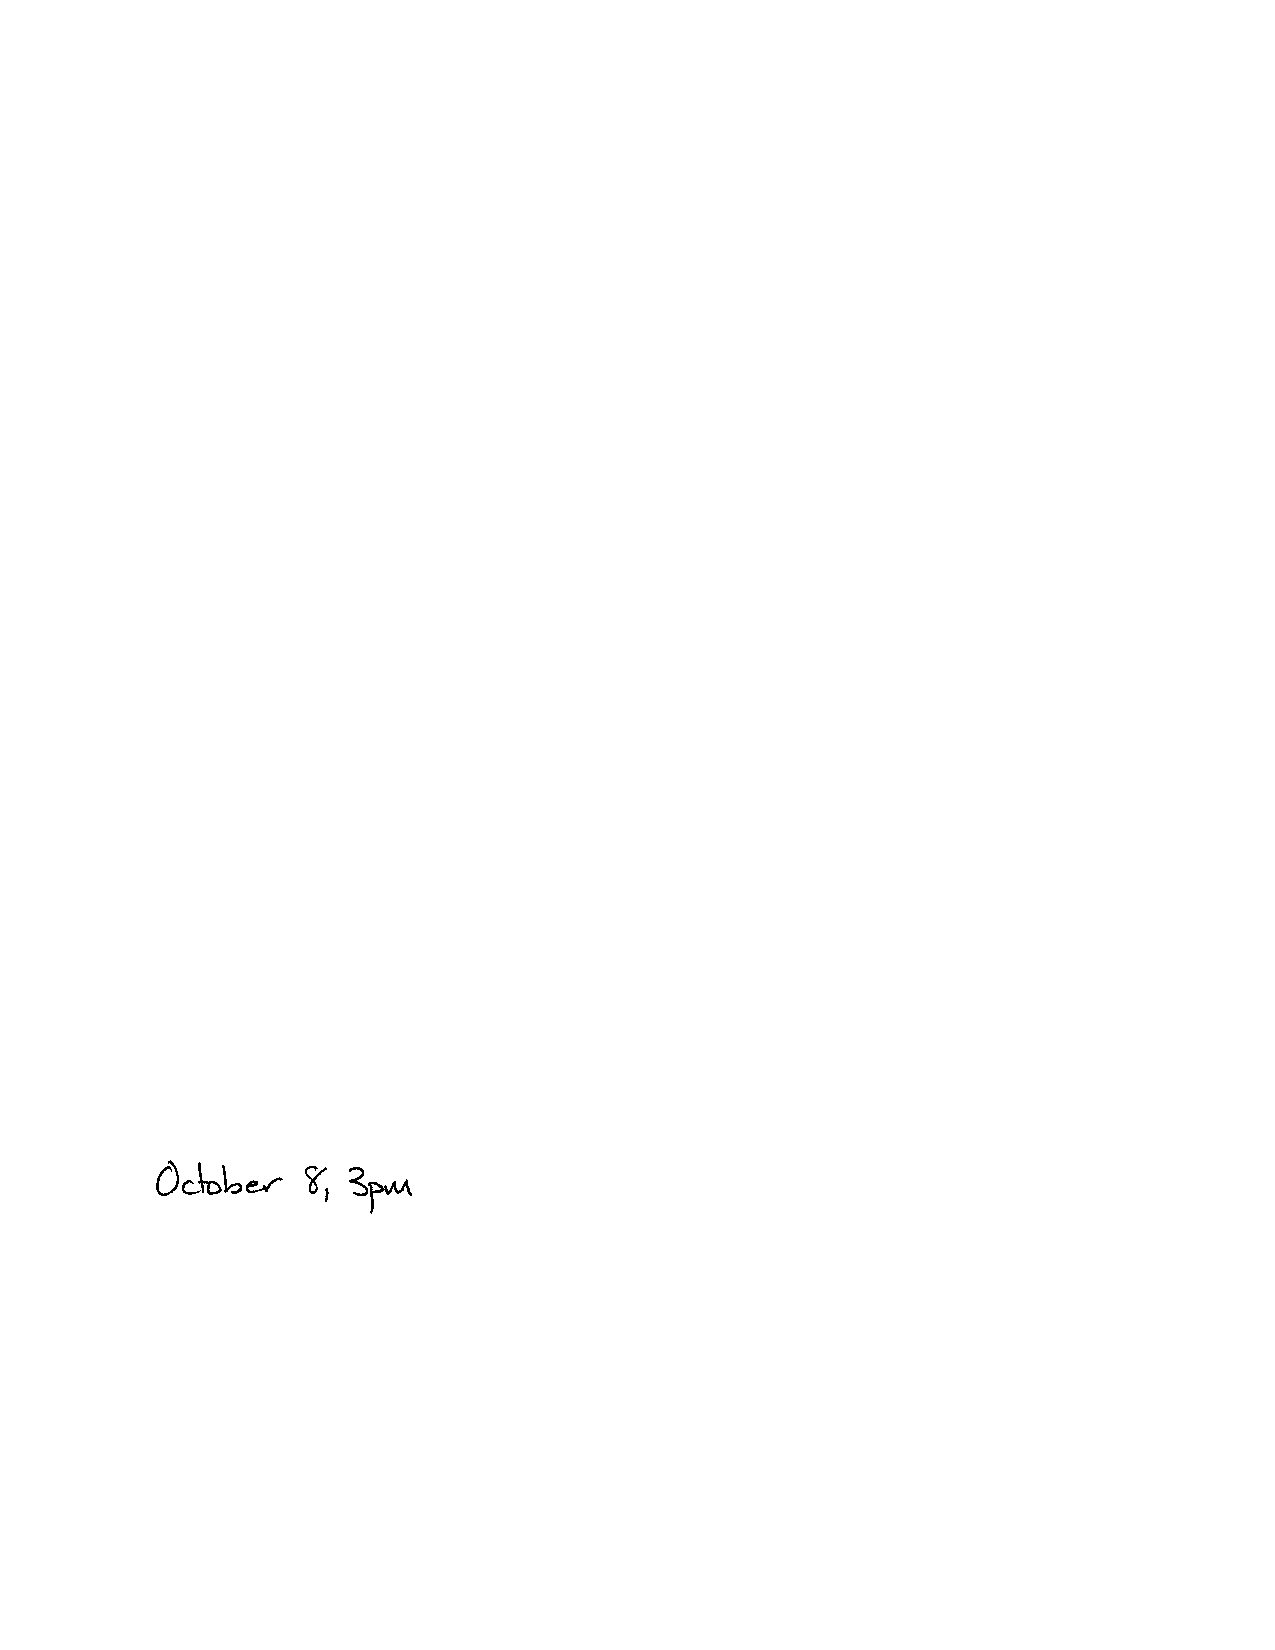
\includegraphics[width=4cm]{date_time}
\\
\textbf{Moon Sketch:} \\
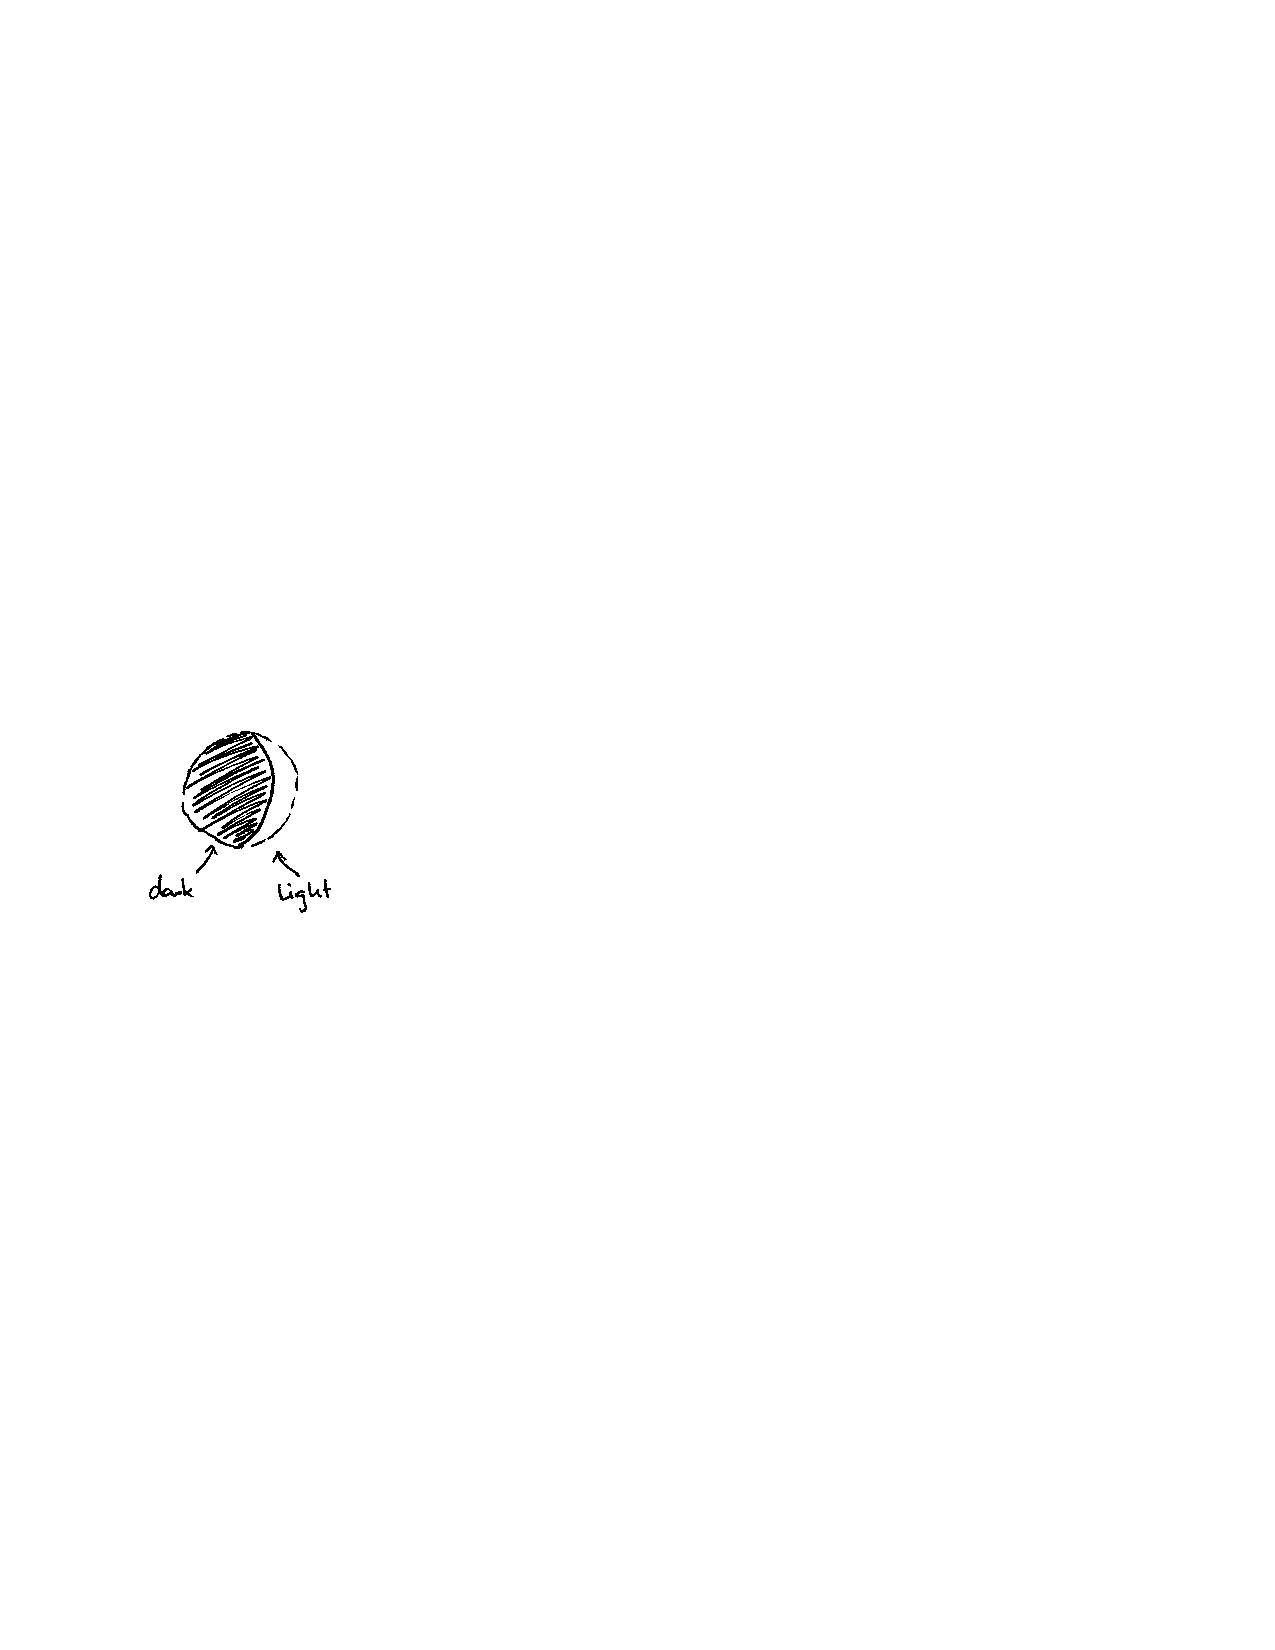
\includegraphics[width=4cm]{moon_sketch}\\
\textbf{Location:} \\
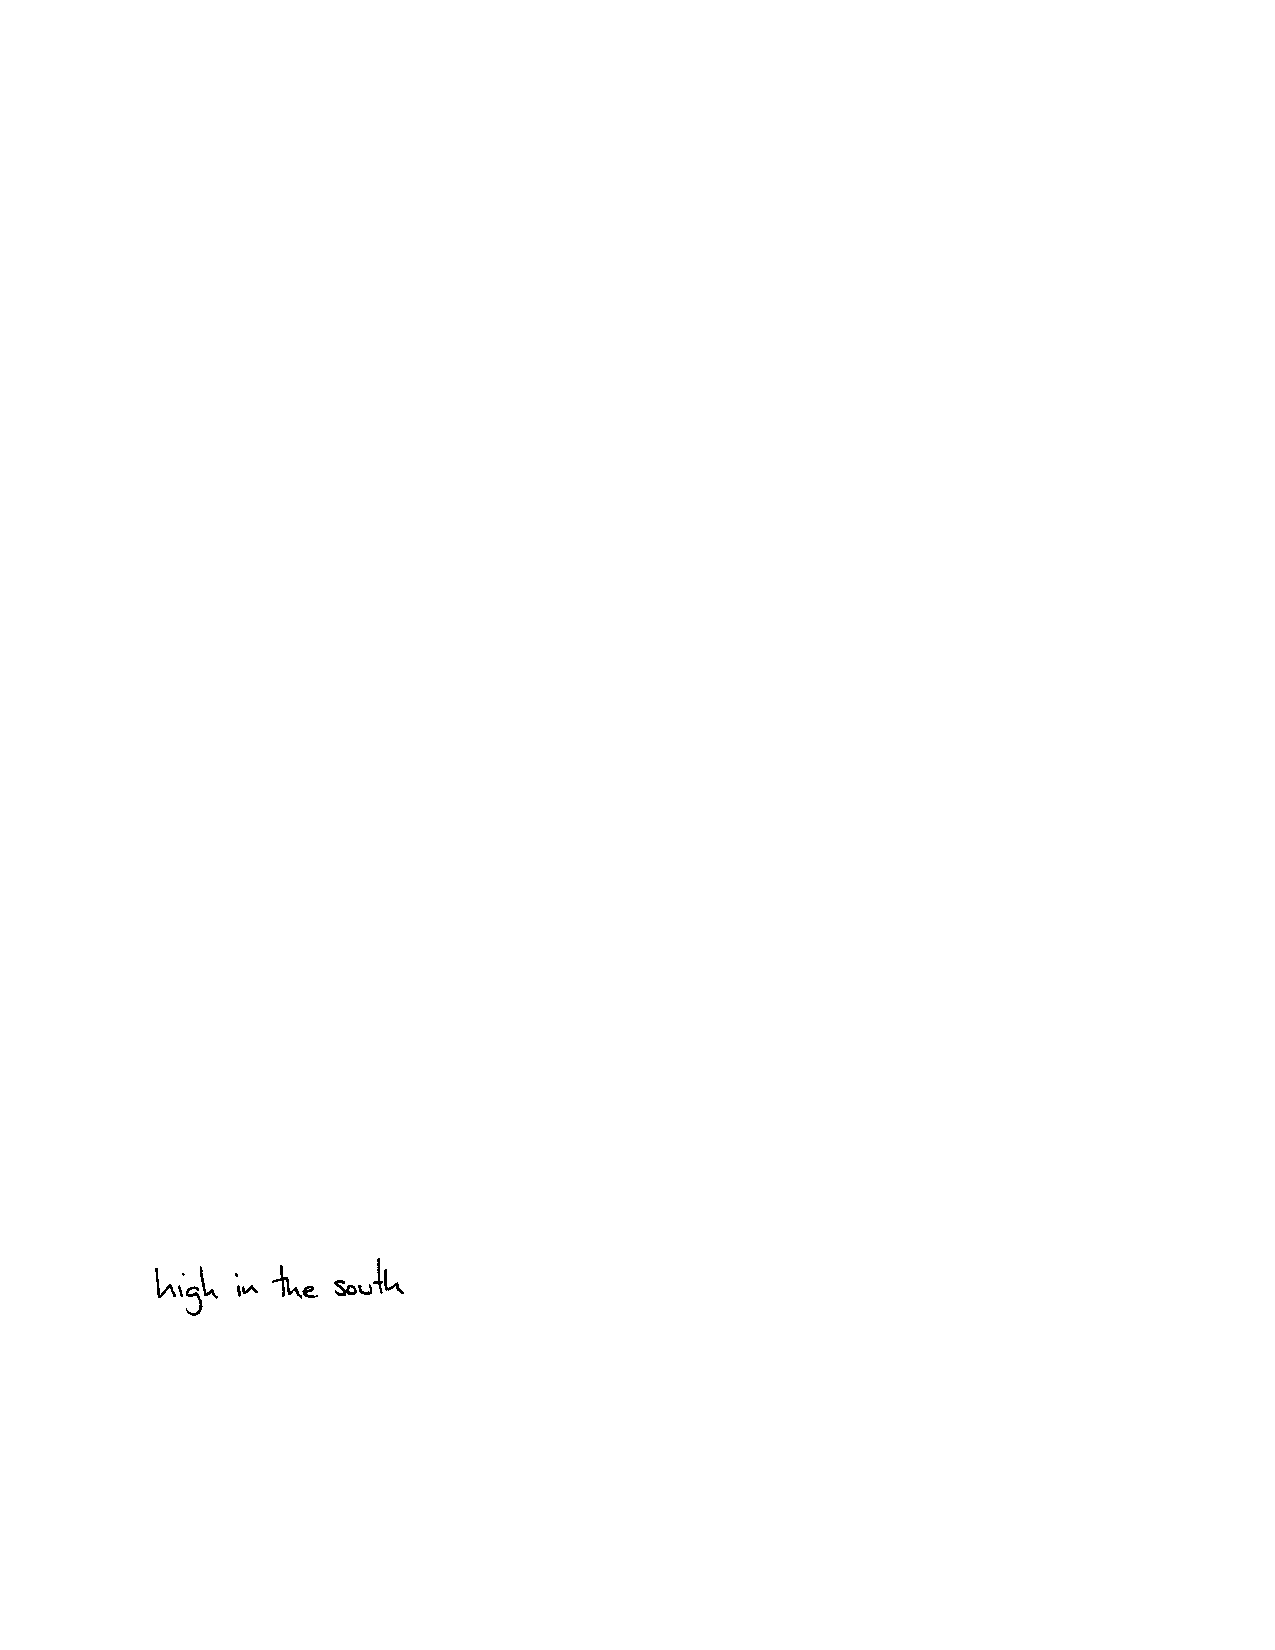
\includegraphics[width=4cm]{location}
\\\hline
\end{tabular}
\end{center}
\end{minipage}
\quad
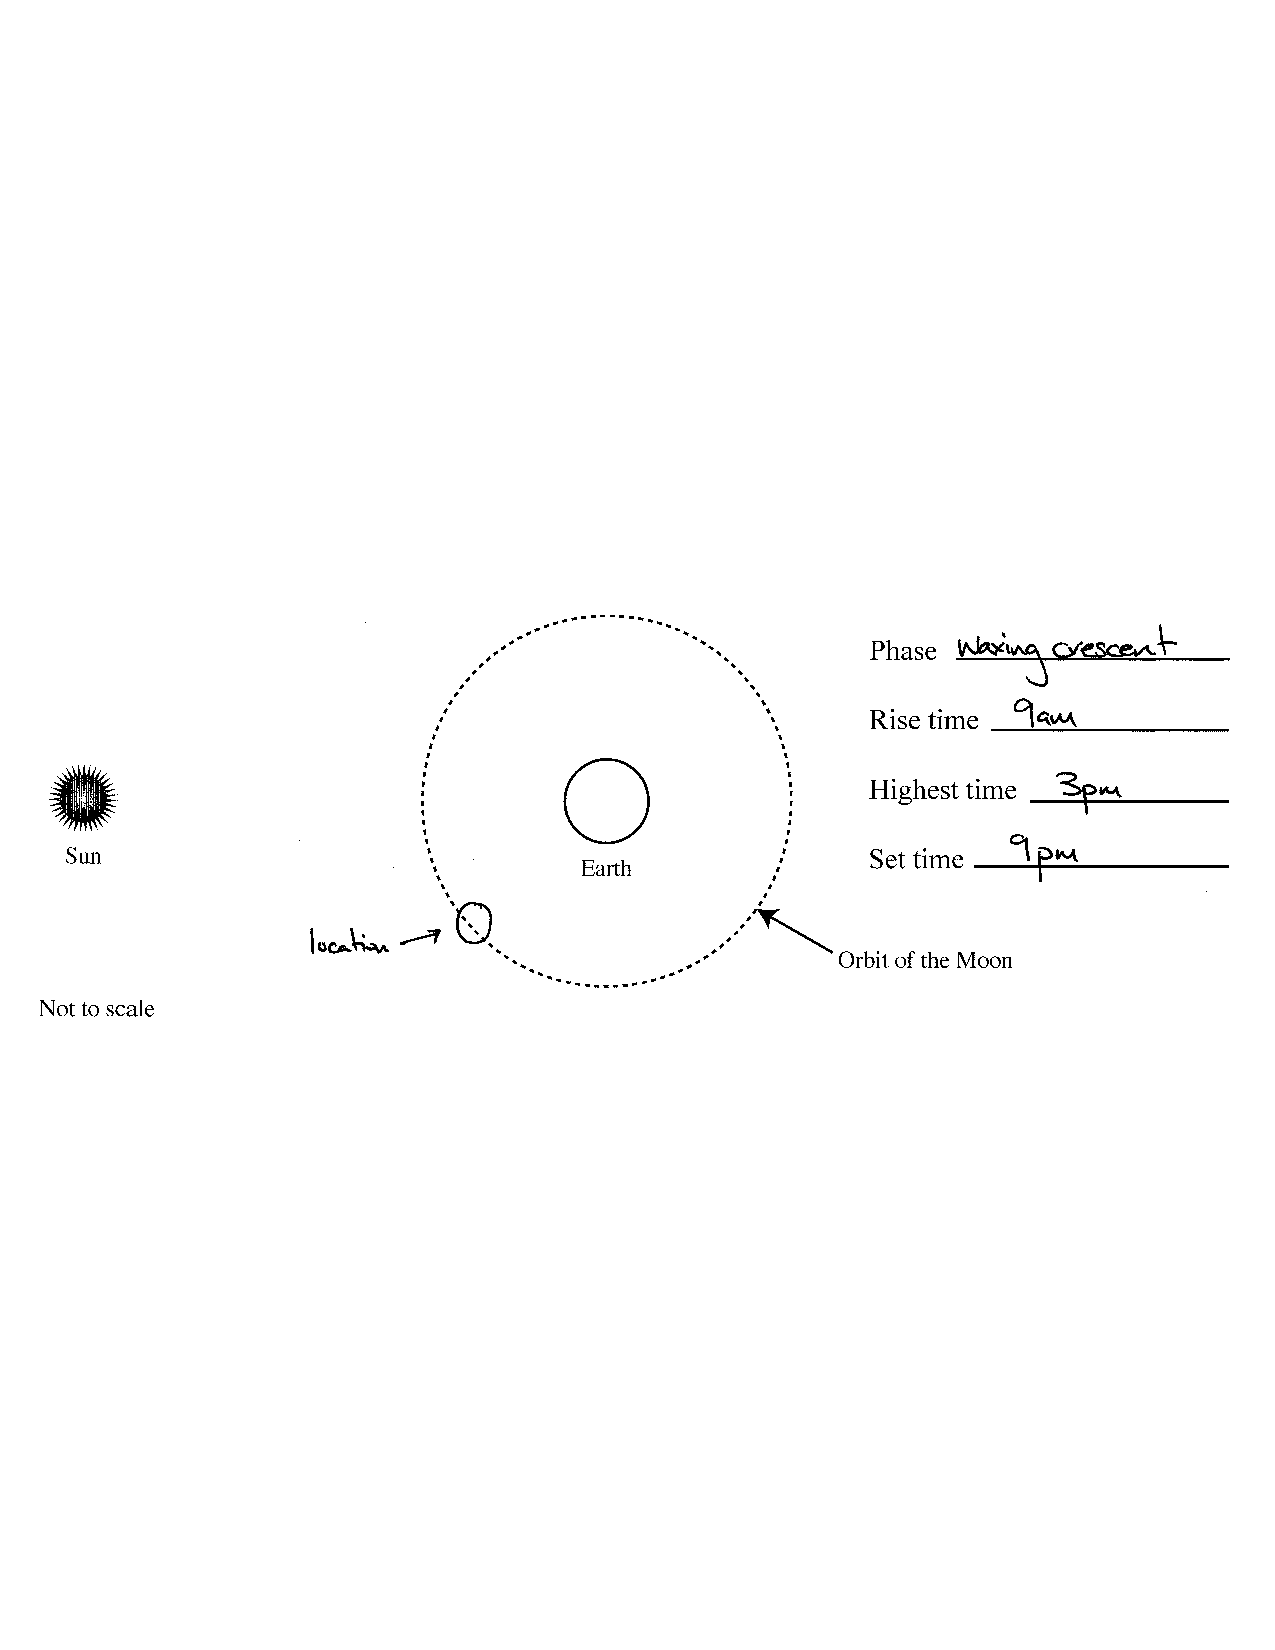
\includegraphics[width=0.7\textwidth]{moon_phase_sketch}

\newpage

\noindent
\begin{minipage}{4.5cm}
\begin{center}
\begin{tabular}{|l|}
\hline 
 \textbf{Observation 1}
 \\
 \hline\hline
\textbf{Date and Time:}\quad\quad\quad\quad\\
\parbox{0.3\linewidth}{\vspace*{1cm}\hspace*{4cm}}
\\
\textbf{Moon Sketch:} \\
\parbox{0.3\linewidth}{\vspace*{3.5cm}\hspace*{4cm}}
\\
\textbf{Location:} \\
\parbox{0.3\linewidth}{\vspace*{1cm}\hspace*{4cm}}
\\\hline
\end{tabular}
\end{center}
\end{minipage}
\begin{minipage}{0.75\textwidth}
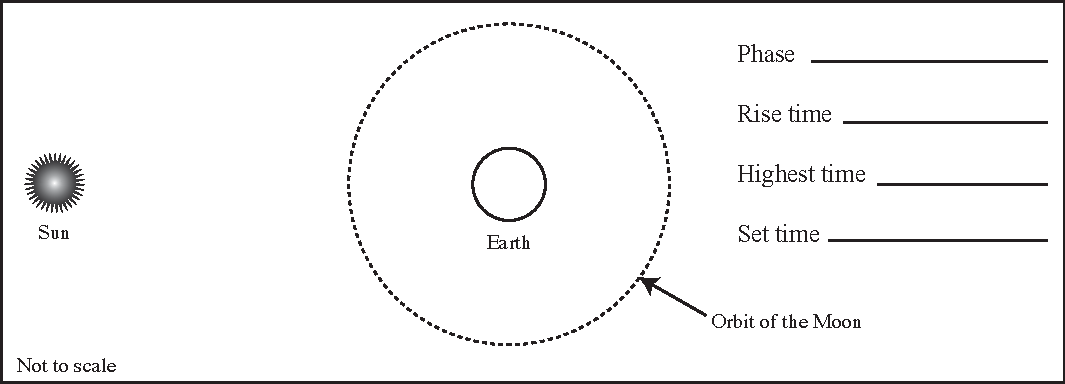
\includegraphics[width=\textwidth]{moon_position_in_orbit_blank}\\
\vspace*{0.5cm}
Is your observation consistent with your sketch? Comment on why.\\

\vspace*{1cm}
\hrulefill
\end{minipage}

\noindent
\begin{minipage}{4.5cm}
\begin{center}
\begin{tabular}{|l|}
\hline 
 \textbf{Observation 2}
 \\
 \hline\hline
\textbf{Date and Time:}\quad\quad\quad\quad\\
\parbox{0.3\linewidth}{\vspace*{1cm}\hspace*{4cm}}
\\
\textbf{Moon Sketch:} \\
\parbox{0.3\linewidth}{\vspace*{3.5cm}\hspace*{4cm}}
\\
\textbf{Location:} \\
\parbox{0.3\linewidth}{\vspace*{1cm}\hspace*{4cm}}
\\\hline
\end{tabular}
\end{center}
\end{minipage}
\begin{minipage}{0.75\textwidth}
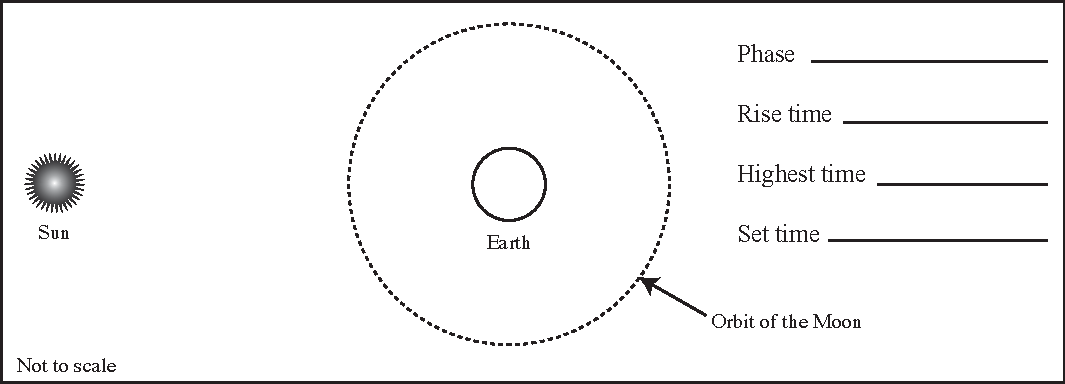
\includegraphics[width=\textwidth]{moon_position_in_orbit_blank}\\
\vspace*{0.5cm}
Is your observation consistent with your sketch? Comment on why.\\

\vspace*{1cm}
\hrulefill
\end{minipage}

\noindent
\begin{minipage}{4.5cm}
\begin{center}
\begin{tabular}{|l|}
\hline 
 \textbf{Observation 3}
 \\
 \hline\hline
\textbf{Date and Time:}\quad\quad\quad\quad\\
\parbox{0.3\linewidth}{\vspace*{1cm}\hspace*{4cm}}
\\
\textbf{Moon Sketch:} \\
\parbox{0.3\linewidth}{\vspace*{3.5cm}\hspace*{4cm}}
\\
\textbf{Location:} \\
\parbox{0.3\linewidth}{\vspace*{1cm}\hspace*{4cm}}
\\\hline
\end{tabular}
\end{center}
\end{minipage}
\begin{minipage}{0.75\textwidth}
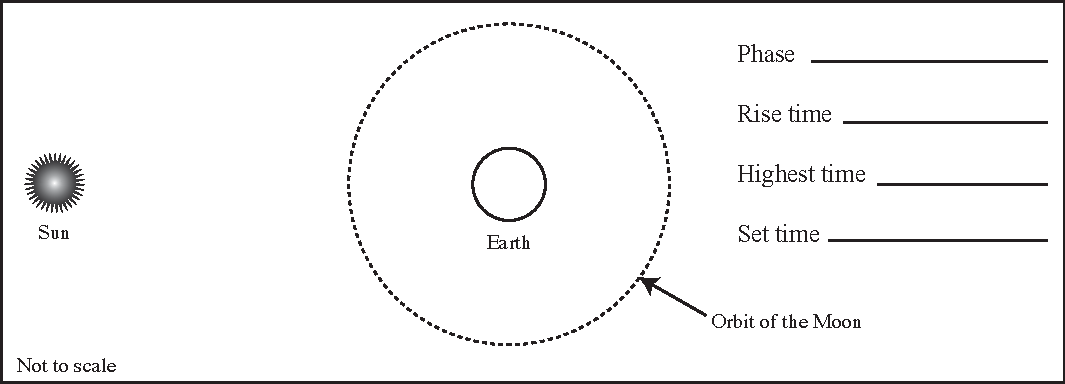
\includegraphics[width=\textwidth]{moon_position_in_orbit_blank}\\
\vspace*{0.5cm}
Is your observation consistent with your sketch? Comment on why.\\

\vspace*{1cm}
\hrulefill
\end{minipage}


\newpage

\section{The Sunset Point}
\label{s:s}

The motion of the Sun on the celestial sphere can be easily detected in
observations of the sunset or sunrise. In this section you will
record the point of sunset three times in a month and compare your observation to the answers to the question in the previous section. On your first evening observing the sun, you will need to make a sketch
of the horizon from your observing location, so make sure you go out 20
minutes before sunset to give yourself chance to complete the sketch before
your first observation. Googling "local sunset" will get you an approximate value
of the sunset time at your current location, but the time you record should be the 
time that you actually see the Sun sink below the horizon.

Choose an observing location with a clear view of the western horizon. All
your observations must be made from exactly the same point, so make a note of
the location you chose below.  Good places to observe on campus are from the
western edge of the Law School plaza, the eastern end of the ESF Quad by the yew trees,
or Mount Olympus; if you are willing to
travel a bit for a nice view, the sunset over Lake Onondaga is usually very nice.

\noindent \textbf{Observing Location:}
\vspace*{0.5cm}

\hrulefill\\
Make a sketch of the horizon from your observation location on page 5 of
this lab packet. To do this, first draw a line in the middle of the page
indicating the horizon (you can rotate the page sideways to give yourself more
space). Now locate two or three easy to identify landmarks on the horizon,
such as water towers, radio masts or distant buildings. You will be measuring
the position of the sunset relative to these objects, so choose some objects
near to and either side of the position of the Sun near sunset time. Mark the
location of these objects on your diagram. Now, using your using your hand as
an angular measuring device, measure the angular separation between the 
distant landmarks you have chosen. Mark the angular separation of these
objects on your diagram.

How are you to measure these angles? A pretty good estimate can be gotten from
your own hand, held at arm's length; people with longer arms tend to have larger 
and longer fingers, which balances out.

\begin{center}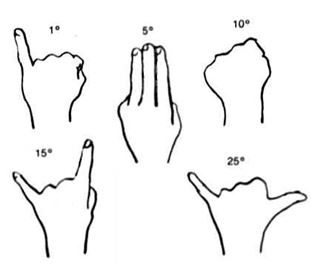
\includegraphics[width=2.5in]{Sky_Angles.jpg}\end{center}

Now wait for the Sun to set. Just as the Sun is setting, mark on your drawing
the point where it goes below the horizon. Label this point with the time and
date of the observation.  Now, using your hand as an angular measuring device,
measure the location of the sunset with respect to a convenient object on the
horizon chosen as reference point. Mark this point on your drawing and report
the angle, together with the time and date, in the first row of the table
below. Mark L or R to indicate if the angle is to the left or to the right of
the landmark.

After one week, return to the same observing location to measure and draw the
location of the sunset point in the same way as above. After one more week has
passed, make a third and final observation. Record your answers in the table
below and on your diagram. When your observations are complete, answer the
questions on the next page.

\begin{center}
\begin{tabular}{|l|l|l|l|l|}
\hline & \parbox[b]{2cm}{\textbf{Date}} & \parbox[b]{2cm}{\textbf{Time}} \quad & \parbox[b]{4cm}{\textbf{Landmark}} & \parbox[b]{3cm}{\textbf{Angle (L or R)}} \\\hline
Observation 1 & \parbox{1cm}{\vspace*{1.7cm}} & & & \\\hline
Observation 2 & \parbox{1cm}{\vspace*{1.7cm}}& & & \\\hline
Observation 3 & \parbox{1cm}{\vspace*{1.7cm}}& & & \\\hline
\end{tabular}
\end{center}


\begin{enumerate}
\item Has the sunset point moved along the horizon?  In which direction?
\vspace*{4cm}

\hrulefill

\item Why did the sunset point move? Why in that direction?
\vspace*{4cm}

\hrulefill
\newpage
\item What is the average daily rate of motion (in degrees per day)? Compare your answer with someone else in your lab who did their measurements earlier or later in the year. Do you get the same answer? Why or why not?

\vspace*{4cm}

\hrulefill

\item In what direction should you look to see the sun rise and set at this
time of the year? Are your observations consistent with this?

\vspace*{4cm}

\hrulefill

\end{enumerate}

\newpage
\section*{Horizon Sketch}

\end{document}


